\section{Problema de investigación y propuesta}

\subsection{Hipótesis}
\begin{frame}[allowframebreaks]
	\frametitle{Hipótesis}
	\begin{tcolorbox}[colback=blue!5,colframe=blue!40!black,title=Hipótesis del trabajo de tesis]
		A partir del relevamiento del estado del arte se establece la hipótesis de que los \textbf{algoritmos de cálculo de similaridad de texto en sitios de CQA}, con el fin de participar del proceso inherente a la aplicación de \textbf{Sistemas de Recomendación} con gran volumen de datos, pueden ser mejorados en cuanto a medidas de rendimiento y de desempeño si se aplica \textbf{un método de ensamble de clustering mediante una arquitectura Big Data} apropiada.
	\end{tcolorbox}

	\framebreak

	\begin{tcolorbox}[colback=blue!5,colframe=blue!40!black,title=Hipótesis del trabajo de tesis (cont.)]
		\bigskip Por tal motivo, y como respuesta a la hipótesis planteada, se presenta:
		\begin{itemize}[<*>]
			\item Un \textbf{desarrollo de un nuevo método de cálculo de similaridad de texto} basado en una \textbf{arquitectura Big Data}.
			\item Una \textbf{aplicación del método a un gran conjunto de datos reales} con el fin de verificar la eficiencia y eficacia del procedimiento.
			\item Un \textbf{análisis comparativo} del método presentado con los algoritmos para cálculo de similaridad de texto del estado del arte.
		\end{itemize}
	\end{tcolorbox}
\end{frame}

\subsection{El método propuesto}
\begin{frame}
	\frametitle{El método propuesto (EQuAL)}
	\begin{figure}
		\centering
		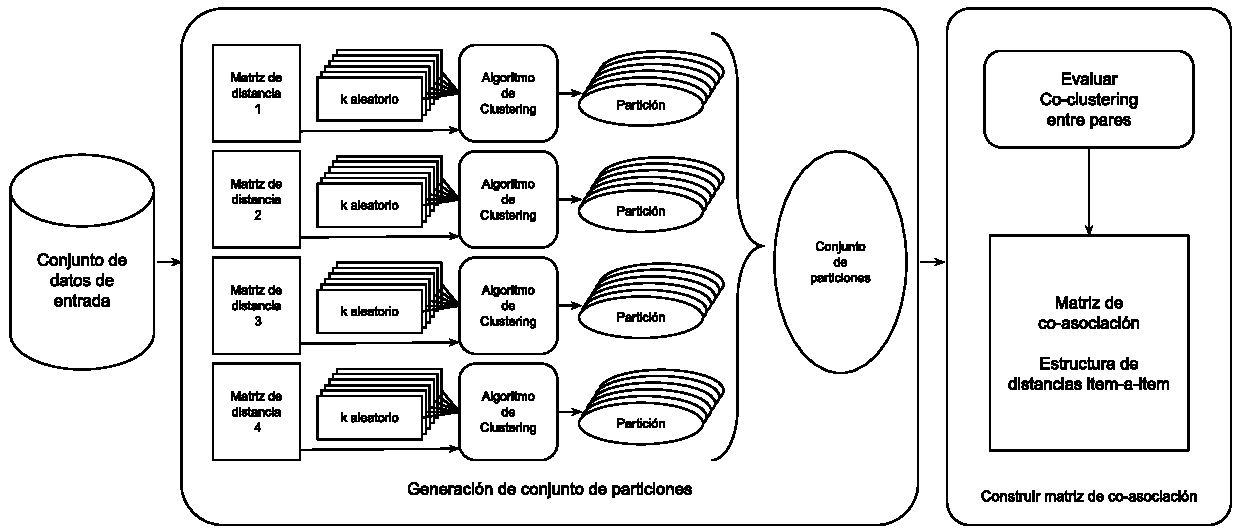
\includegraphics[width=0.9\linewidth]{../8_problema_investigacion/imagenes/metodo_equal}
		\label{fig:metodoequal}
	\end{figure}
\end{frame}

\subsection{Arquitectura de procesamiento de datos}
\begin{frame}
	\frametitle{Arquitectura de procesamiento de datos}
	\begin{figure}
		\centering
		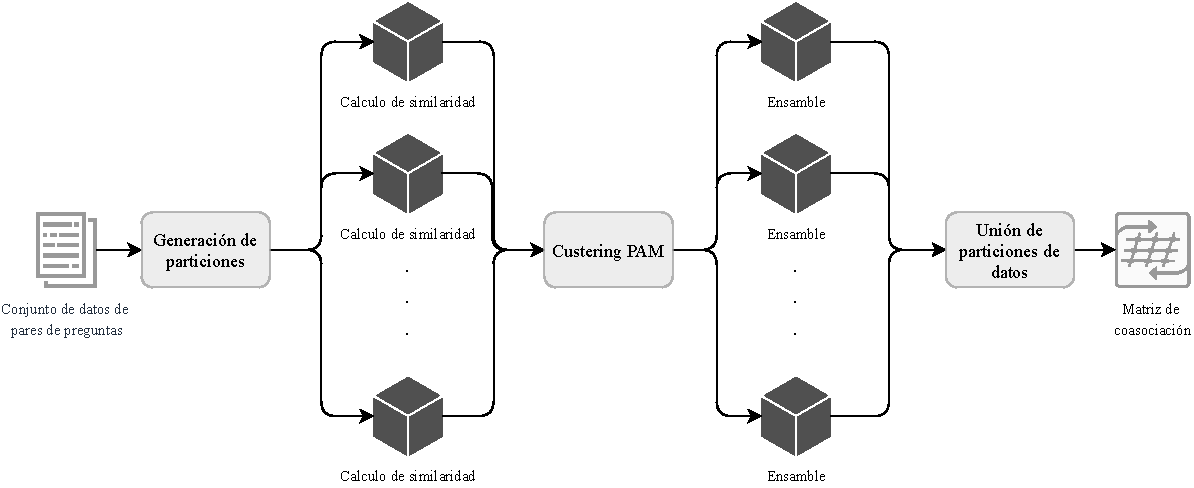
\includegraphics[width=0.9\linewidth]{../8_problema_investigacion/imagenes/equal_distribuido}
		\label{fig:equaldistribuido}
	\end{figure}
\end{frame}

\subsection{Implementación en un sistema de recomendación de tiempo real}
\begin{frame}
	\frametitle{Implementación en un sistema de recomendación de tiempo real}
	\begin{figure}
		\centering
		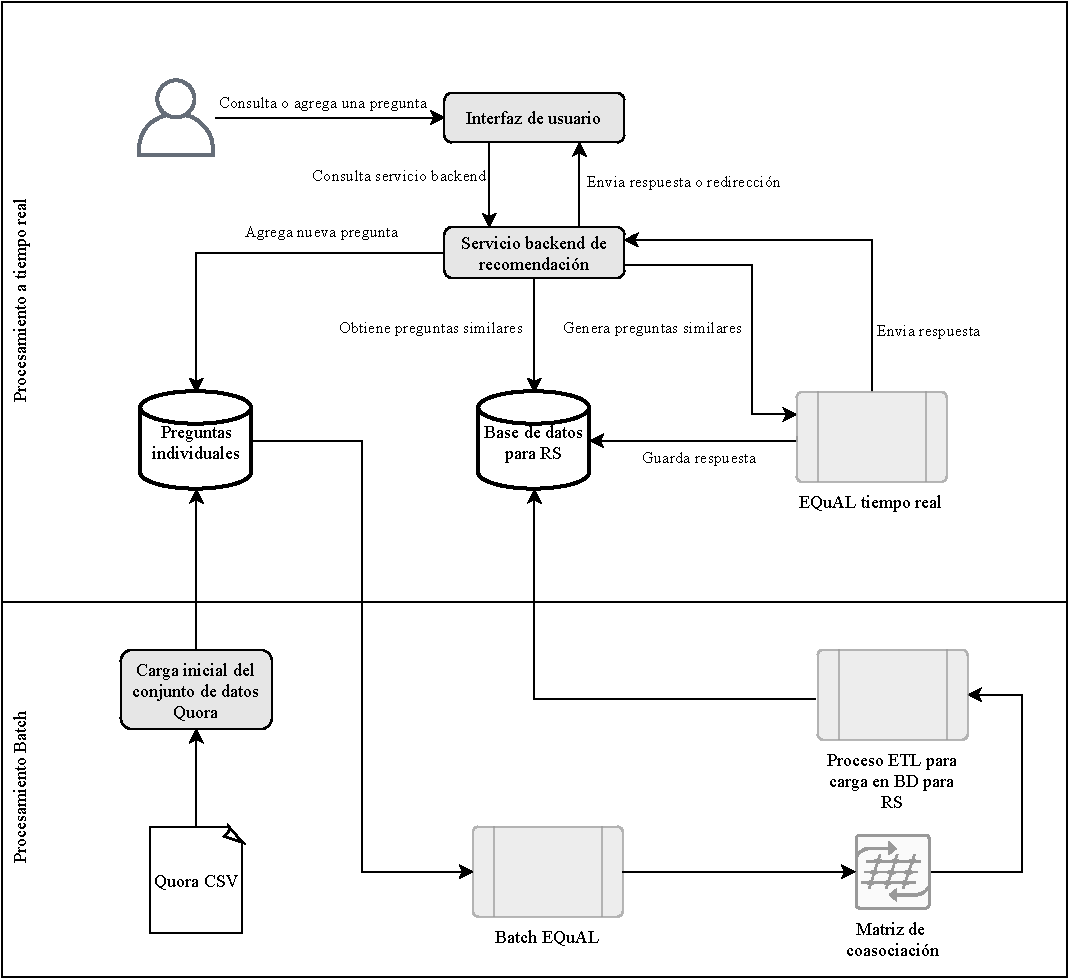
\includegraphics[width=0.55\linewidth]{../8_problema_investigacion/imagenes/implementacion_rs}
		\label{fig:implementacionrs}
	\end{figure}
\end{frame}